\chapter{Introdução}
\label{chap:introducao}

\lipsum[2]

\begin{figure}[h!]
	\caption{Mapa conceitual do estudo da história e relações com o objeto de estudo}
	\label{fig_mapa}
	\begin{center}
		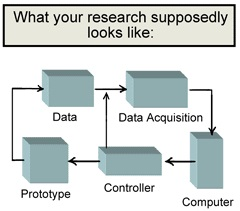
\includegraphics[width=8cm]{capitulos/figuras/figura-1}		
	\end{center}
	\fontedafigura{8cm}{os autores}
\end{figure}

\lipsum[2]
\lipsum[2]
\lipsum[2]

\begin{figure}[h!]
	\caption{Paradigma segundo processos que caracterizam a EFSFVS como Escola do SUS}
	\label{fig_paradigma}
	\begin{center}
		
\includegraphics[width=8cm]{capitulos/figuras/figura-2}
	\end{center}
	\fontedafigura{8cm}{Adaptado de}
\end{figure}

\lipsum[2]
\lipsum[2]

\section{Motivação}
\lipsum[2]
\lipsum[2]

\section{Objetivos}

\lipsum[2]
\lipsum[2]
\lipsum[2]
\lipsum[2]
\lipsum[2]
\begin{table}[h!]	
	\caption{Internal exon scores}
	\label{tab:internal}
	\centering
	\begin{tabular}{|c|l|l|}
		\hline
		Ranking & Exon Coverage & Splice Site Support\\
		\hline
		E1 & Complete coverage by a single transcript & Both splice sites\\
		E2 & Complete coverage by more than a single transcript & Both splice sites\\
		E3 & Partial coverage & Both splice sites\\
		E4 & Partial coverage & One splice site\\
		E5 & Complete or partial coverage & No splice sites\\
		E6 & No coverage & No splice sites\\
		\hline
	\end{tabular}
	\fontedatabela{14.6cm}{os autores}
\end{table}

\lipsum[2]
\subsection{Objetivo Geral}
\lipsum[2]

\subsection{Objetivos Específicos}
	\lipsum[2]
	
	\begin{alineas}
		\item \lipsum[2]
		\item \lipsum[2]
		\begin{alineas}
			\item \lipsum[2]
			\item \lipsum[2]
		\end{alineas}
		\item \lipsum[2]	
	\end{alineas}
	
	\lipsum[2]
\subsubsection{Objetivo Geral}
	\lipsum[2]
	\cite{lamport1986latex} e \cite{wessberg2000real} e \cite{knuth} e \cite{lamport} e \cite{Maia2011} e \cite{mortalidade}
	
\subsubsection{Objetivo Geral}
	\lipsum[2]
	\acrlong{DATASUS},\acrlong{DNV},\acrlong{DO},\acrlong{ESF},\acrlong{IBGE},\acrlong{MFC},\acrlong{MI},\acrlong{MS},\acrlong{NV},\acrlong{ODM},\acrlong{OI},\acrlong{OMS},\acrlong{ONU},\acrlong{PNI},\acrlong{PSF},\acrlong{RIPSA},\acrlong{RN},\acrlong{SIM},\acrlong{SINASC},\acrlong{SUS},\acrlong{TMI},\acrlong{TMMFC}
	